%%%%%%%%%%%%%%%%%%%%%%%%%%%%%%%%%%%%%%%%%%%%%%%%%%%%%%%%%%
\section{Representation}
\label{sec:representation}
%%%%%%%%%%%%%%%%%%%%%%%%%%%%%%%%%%%%%%%%%%%%%%%%%%%%%%%%%%

%This section: CCG representation, including types, the grammar.
In this section, we first define our type system, then discuss our lexicon, then describe how we parse. Our system takes a three-step parsing approach. First, we use a CCG parser to build a set base parses for each temporal phrase in isolation (where each base parse is referred to a a context-independent parse). Then, for each context-independent parse, we deterministically build five context-dependent parses. Once we select a single parse from the set of candidate context-depndent parses (which we discuss in the section titled Learning), we execute the parse to ground to a final representation.

%%%%%%%%%%%%%%%%%%%%%%%%%%%%%%%%%%%%%%%%%%%%%%%%%%%%%%%%%%
\subsection{Types within CCG}
\label{sec:CCGtypes}
%%%%%%%%%%%%%%%%%%%%%%%%%%%%%%%%%%%%%%%%%%%%%%%%%%%%%%%%%%
We define five 

\begin{definition}[Range]
A range is a period between two times. For example, \emph{June 13th, 2013}, \emph{today}, and \emph{1987} all ground to ranges.
\end{definition}

\begin{definition}[Sequence] 
A sequence represents an infinite sequence of ranges. For example, \emph{each Thursday} grounds to a range. The duration between each range in a sequence is the same. In the example \emph{each Thursday}, there is a week between each range. Sequences are represented as under-specified ranges. If we were interested in grounding the phrase \emph{June 13th, 2013}, we could first ground \emph{June 13th} to the sequence of all June 13ths, which we could represent as XXXX-6-13, i.e. June 13th of an unspecified year.
\end{definition}

\begin{definition}[Duration]
A duration is a period of time with no specified start or end dates. For example, \emph{two months}, \emph{three years}, and \emph{one day} all ground to durations of time. 
\end{definition}

\begin{definition}[Number]
Numbers only appear in logical forms, never in fully executed output. Numbers are necessary when grounding durations, such as \emph{4 years}, \emph{1 hour}, or \emph{3 weeks}. 
\end{definition}

\begin{definition}[Functional Types]
There are a number of functional types, all of arity less than or equal to two. They are fully outlined in a table in section TODO PUT SECTION HERE
\end{definition}

%%%%%%%%%%%%%%%%%%%%%%%%%%%%%%%%%%%%%%%%%%%%%%%%%%%%%%%%%%
\subsection{Lexicon}
%%%%%%%%%%%%%%%%%%%%%%%%%%%%%%%%%%%%%%%%%%%%%%%%%%%%%%%%%%
A CCG is defined by a lexicon and set of combinators. In this work, we use standard forward and backward application with a hand-built lexicon to build our base parses. 

\begin{figure}[t!]
   \center
   {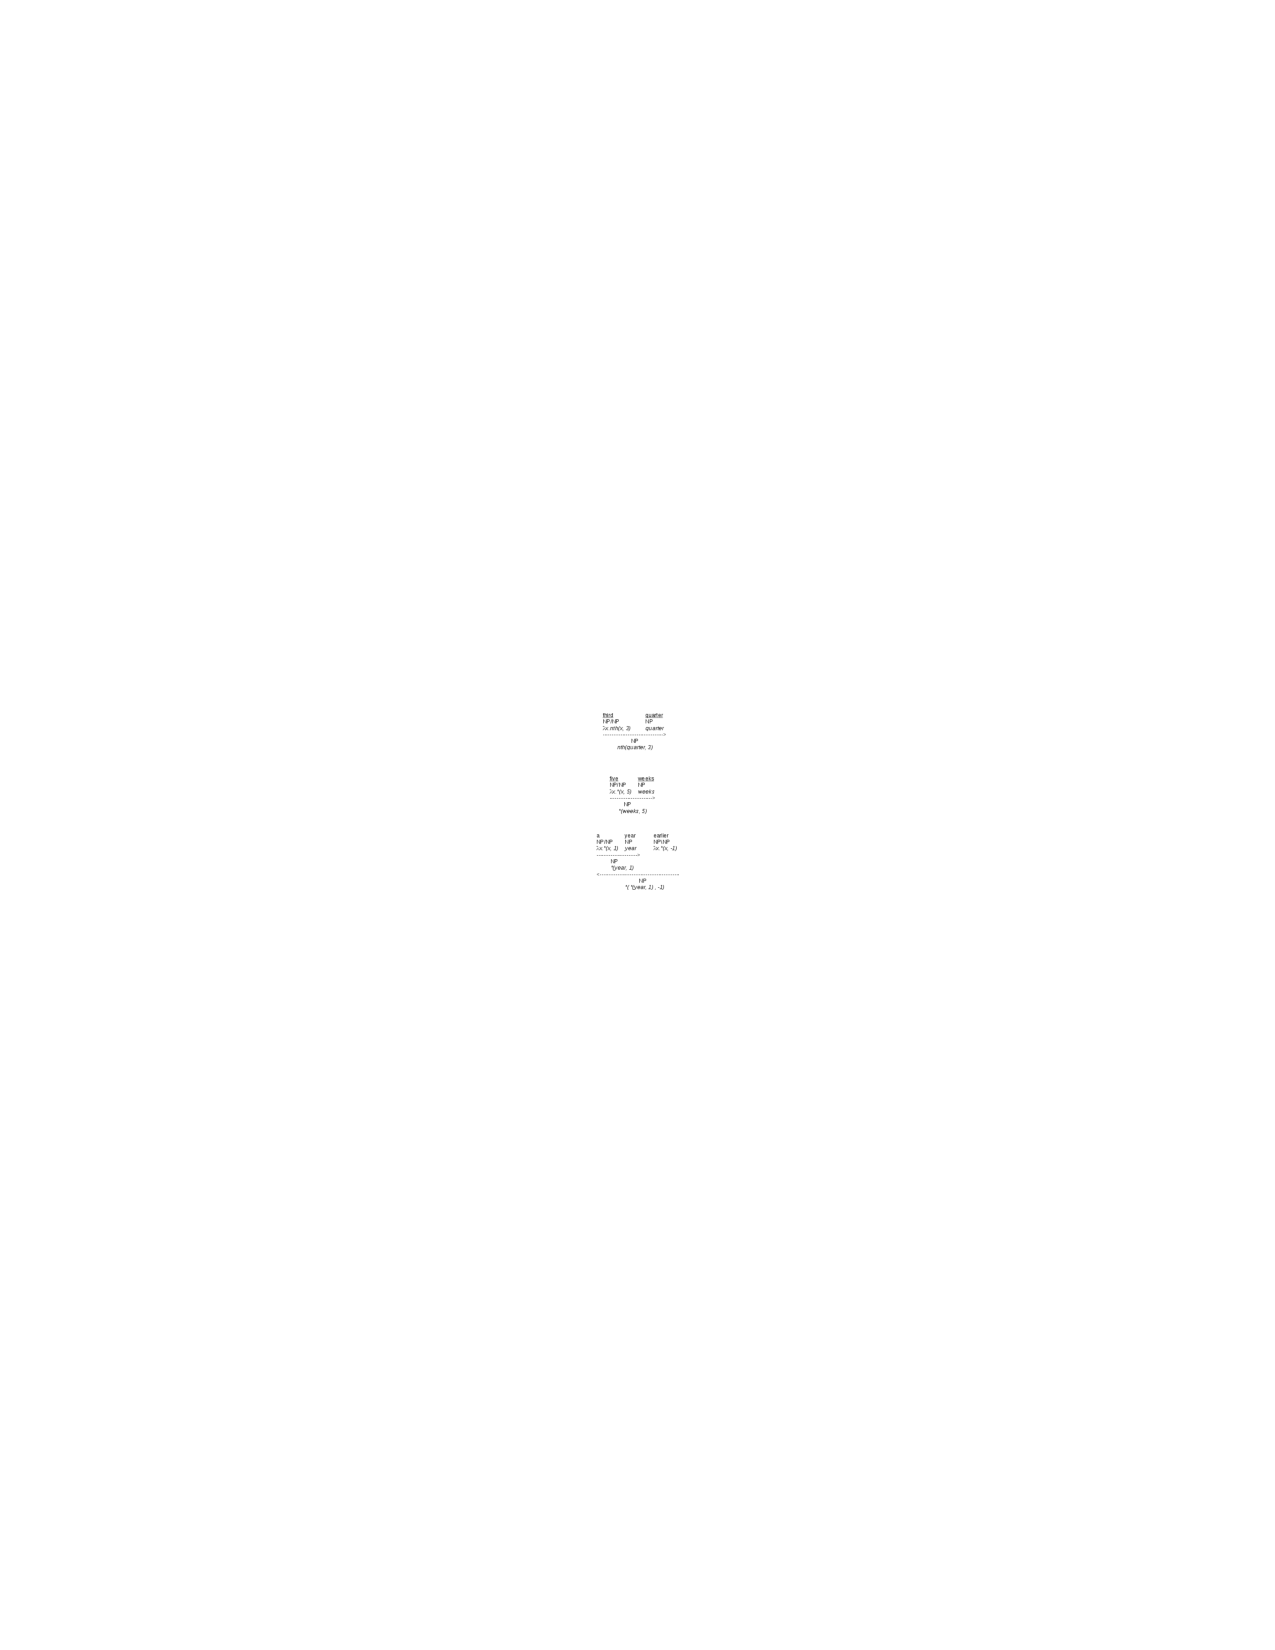
\includegraphics[width=0.95\columnwidth]{fig/lexiconExample.pdf}}
   \caption{Above we can see three example parses. Each of these parses represents a base parse for the given temporal phrase. We can see how the base parse is built from the individual categories drawn from the lexicon. In the first example, we are parsing the phrase \emph{third quarter}. The entries in the lexicon that are being used in this parse are $\lambda x.nth(x,3)$ and $quarter$, which correspond to \emph{third} and \emph{quarter}, respectively. These combine to create the base parse for the first phrase, $nth(quarter,3)$. 
The second example is very similar to the frist. However, the third example first does forward composition (combining $\lambda x*(x,1)$ with $year$) then does backward composition (combining $\lambda x.*(x,-1)$ with $*(year,1)$). 
The first context-independent parse, $nth(quarter,3)$ represents the sequence of all third quarters, which needs additional logic to be correctly ground to a single third quarter. The second parse, $*(weeks, 5)$, can be fully ground to a duration of five weeks without needing an additional context step. The third parse, $*(*(year,1),-1)$, can't actually be ground to a date at all without additional contextual information. 
   } 
   \label{fig:language-venn}
\end{figure}


%%%%%%%%%%%%%%%%%%%%%%%%%%%%%%%%%%%%%%%%%%%%%%%%%%%%%%%%%%
\subsection{Pasing Using CCG}
%%%%%%%%%%%%%%%%%%%%%%%%%%%%%%%%%%%%%%%%%%%%%%%%%%%%%%%%%%
First, for each temporal phrase in our dataset, we use a CKY parser to get a set of CCG logical forms. These are built only from the phrase itself, and don't take any additional information into account. Some ranges can be fully ground without looking at the context in which they appear, such as \emph{June 6th, 2013}. Similarly, durations such as \emph{five weeks} or \emph{a year} don't need to look at surrounding context to be executed to a final form. However, the majority of phrases do require some context to ground fully. Phrases such as \emph{Friday} are parsed to logic that represents sequences, in this case the sequence of all Fridays. To ground phrases such as those to a single range, we need to look at context. 
%%%%%%%%%%%%%%%%%%%%%%%%%%%%%%%%%%%%%%%%%%%%%%%%%%%%%%%%%%
\subsection{Building Context-Dependent Parse}
%%%%%%%%%%%%%%%%%%%%%%%%%%%%%%%%%%%%%%%%%%%%%%%%%%%%%%%%%%
From each context-independent logical form we get from the base CCG parser, we use a deterministic process to build a set of five context-dependent logical forms. These represent the five possible groundings of each of our base parses. For fully-sepcified ranges and for durations, we don't actually need to change the logical form, so the frist of the the context-dependent logical forms is an unchanged version of the context-independent logical form. Sequences often represent an infinite number of ranges, such as $nth(quarter,3)$. We can ground these sequences to one of three ranges, either the range before the document was published, the range after the document was published, or the range during which the document was published. Finally, for a class of temporal phrases that refer to a previously uttered temporal phrase, such as \emph{a year earlier}, we build a logical form that grounds the current phrase based on the previous one. An example is shown in the figure above.

%%%%%%%%%%%%%%%%%%%%%%%%%%%%%%%%%%%%%%%%%%%%%%%%%%%%%%%%%%
\subsection{Building Context-Dependent Parse}
%%%%%%%%%%%%%%%%%%%%%%%%%%%%%%%%%%%%%%%%%%%%%%%%%%%%%%%%%%














